\section{Experimental Results}\label{s:results}

\subsection{Histograms}\label{ss:results-histograms}


\begin{figure}[H]
\centering
\centerline{
\begin{minipage}{.5\linewidth}
  \centering
  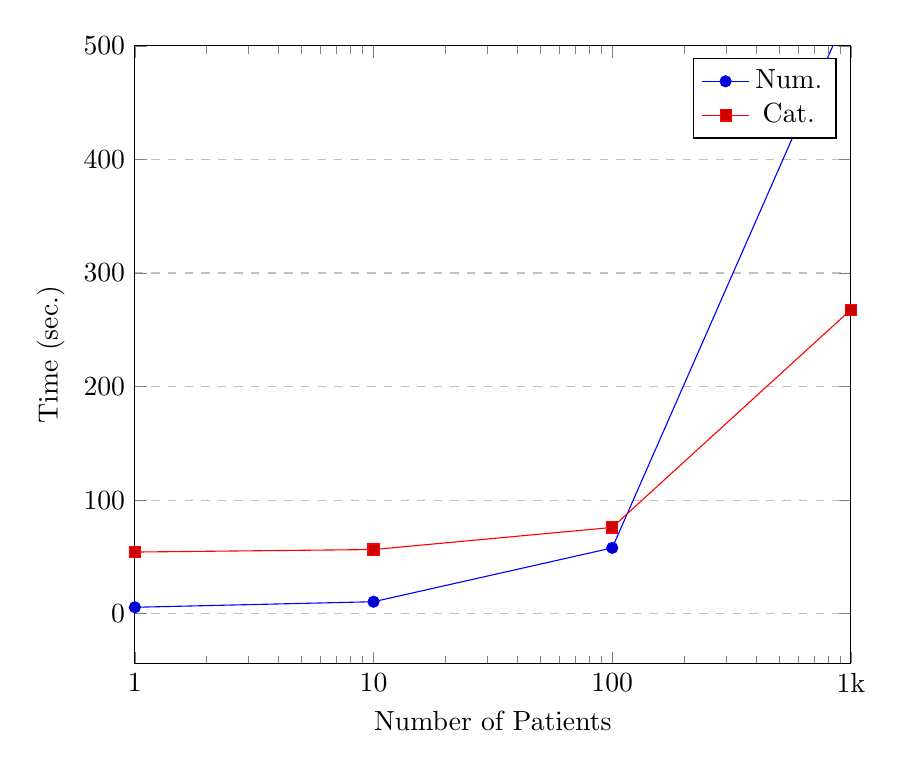
\begin{tikzpicture}
  \begin{axis}[scale only axis, enlarge x limits=-1, width=\textwidth*0.75, ymajorgrids=true, xmode=log, log ticks with fixed point, xlabel={Number of Patients}, ylabel={Time (sec.)}, xticklabels={1,10,100,1k}, ymax=500, grid style=dashed]
  \addplot
      coordinates {(1, 5.66)(10, 10.54)(100, 57.94)(1000, 536.09)};
  \addlegendentry{Num.}
  \addplot
      coordinates {(1, 54.29)(10, 56.5)(100, 75.95)(1000, 267.7)};
  \addlegendentry{Cat.}
  \end{axis}
  \end{tikzpicture}
  \caption{1-Dimensional histograms timings}
\end{minipage}%
\begin{minipage}{.5\linewidth}
  \centering
  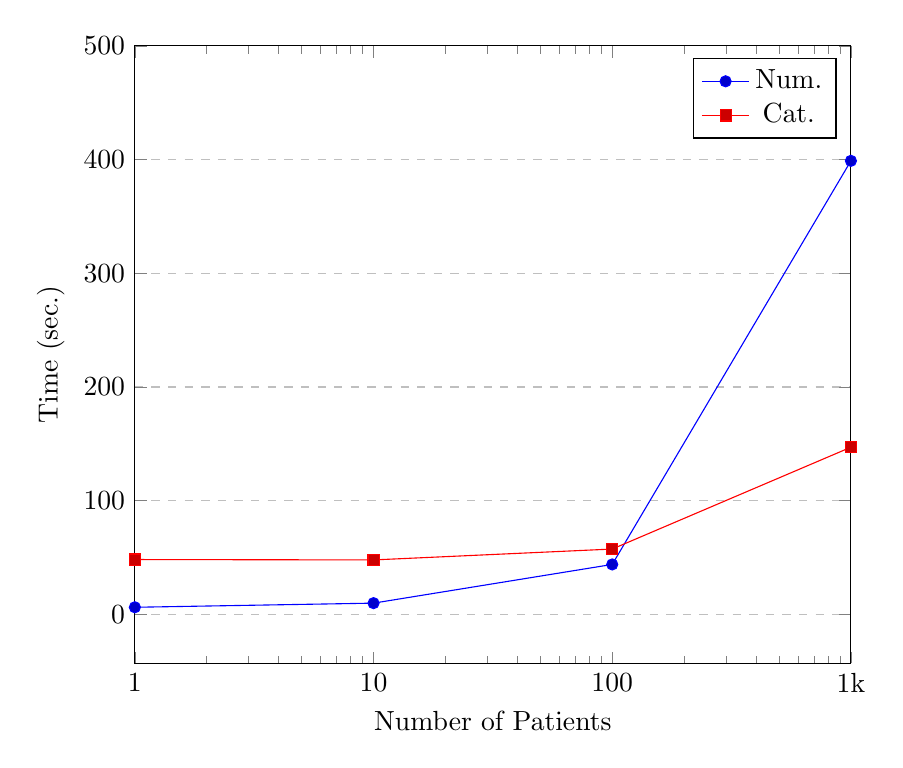
\begin{tikzpicture}
  \begin{axis}[scale only axis,enlarge x limits=-1,width=\textwidth*0.75,ymajorgrids=true,xmode=log,log ticks with fixed point,xlabel={Number of Patients},ylabel={Time (sec.)},xticklabels={1,10,100,1k},ymax=500,grid style=dashed]
  \addplot
      coordinates {(1, 6.36)(10, 9.99)(100, 44.02)(1000, 398.86)};
  \addlegendentry{Num.}
  \addplot
      coordinates {(1, 48.33)(10, 47.99)(100, 57.55)(1000, 147.08)};
  \addlegendentry{Cat.}
  \end{axis}
  \end{tikzpicture}
  \caption{2-Dimensional histograms timings}
\end{minipage}
}
\end{figure}


%%%%%%%%%%%%%%%%%%%%%%%%%%%%%%%%%%%%%%%%%%%%%%%%%%%%%%%%%%%%%%%%%%%%%%%%%%%%%%%%%%%

\begin{figure}[H]
\centering
\centerline{
\begin{minipage}{.5\linewidth}
  \centering
  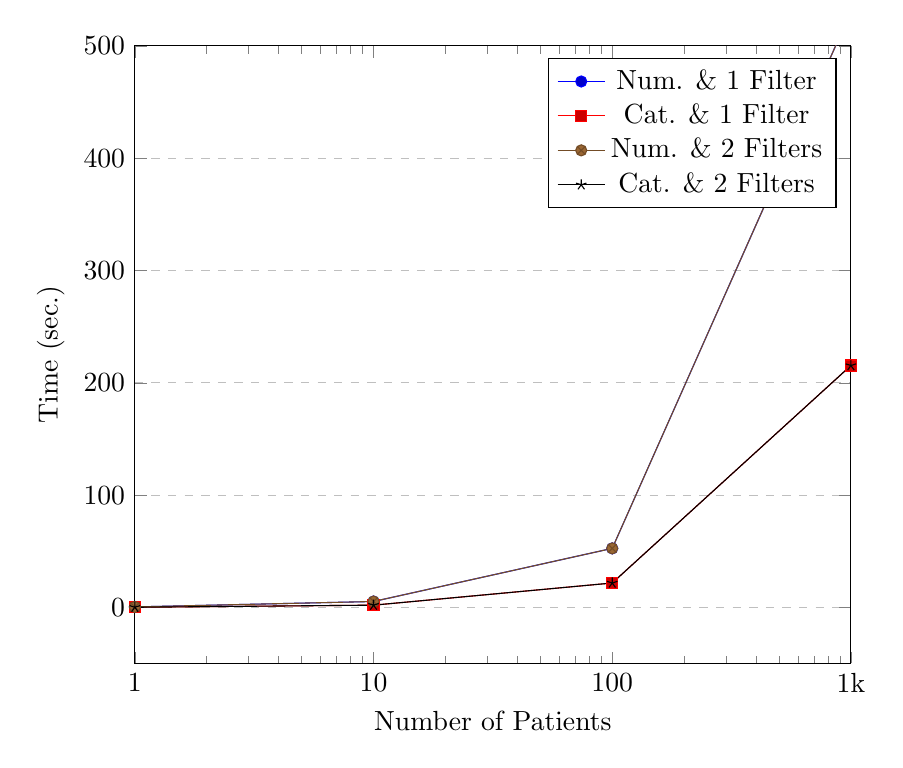
\begin{tikzpicture}
  \begin{axis}[scale only axis, enlarge x limits=-1, width=\textwidth*0.75, ymajorgrids=true, xmode=log, log ticks with fixed point, xlabel={Number of Patients}, ylabel={Time (sec.)}, xticklabels={1,10,100,1k}, ymax=500, grid style=dashed]
  \addplot
      coordinates {(1, 0.548186)(10, 5.381935)(100, 52.661779)(1000, 530.589239)};
  \addlegendentry{Num. \& 1 Filter}
  \addplot
      coordinates {(1, 0.237847)(10, 2.117192)(100, 21.845599)(1000, 215.412621)};
  \addlegendentry{Cat. \& 1 Filter}
  \addplot
      coordinates {(1, 0.548186)(10, 5.381935)(100, 52.661779)(1000, 530.589239)};
  \addlegendentry{Num. \& 2 Filters}
  \addplot
      coordinates {(1, 0.237847)(10, 2.117192)(100, 21.845599)(1000, 215.412621)};
  \addlegendentry{Cat. \& 2 Filters}
  \end{axis}
  \end{tikzpicture}
  \caption{1-Dimensional histograms with filters timings}
\end{minipage}%
\begin{minipage}{.5\linewidth}
  \centering
  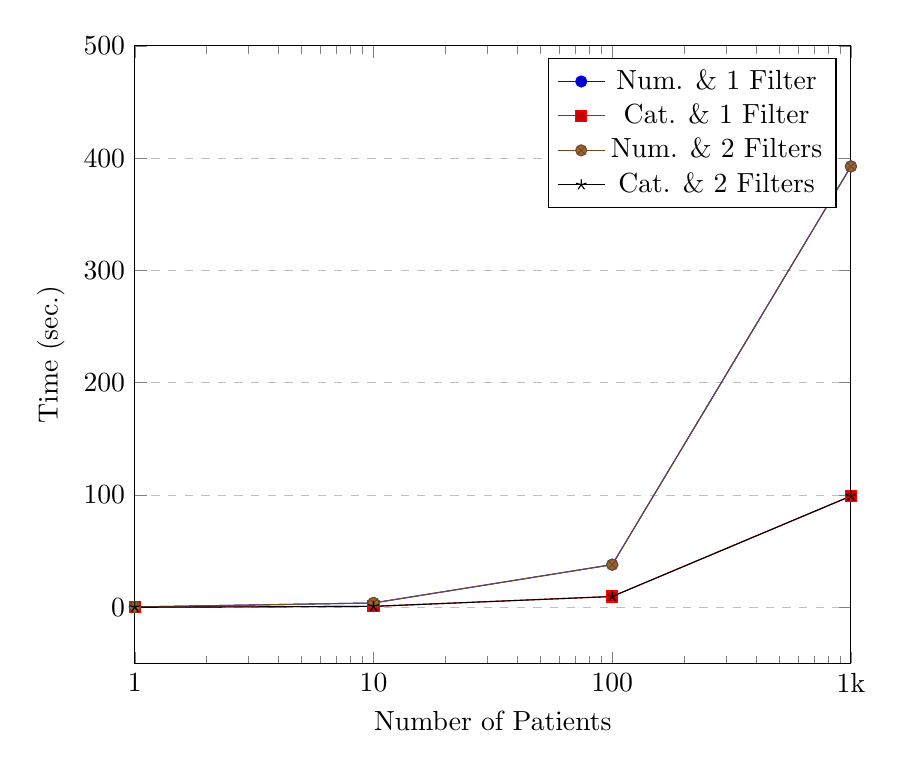
\begin{tikzpicture}
  \begin{axis}[scale only axis,enlarge x limits=-1,width=\textwidth*0.75,ymajorgrids=true,xmode=log,log ticks with fixed point,xlabel={Number of Patients},ylabel={Time (sec.)},xticklabels={1,10,100,1k},ymax=500,grid style=dashed]
  \addplot
      coordinates {(1, 0.382224)(10, 3.947421)(100, 38.052168)(1000, 392.634467)};
  \addlegendentry{Num. \& 1 Filter}
  \addplot
      coordinates {(1, 0.099595)(10, 0.922558)(100, 9.712436)(1000, 99.149262)};
  \addlegendentry{Cat. \& 1 Filter}
  \addplot
      coordinates {(1, 0.382224)(10, 3.947421)(100, 38.052168)(1000, 392.634467)};
  \addlegendentry{Num. \& 2 Filters}
  \addplot
      coordinates {(1, 0.099595)(10, 0.922558)(100, 9.712436)(1000, 99.149262)};
  \addlegendentry{Cat. \& 2 Filters}
  \end{axis}
  \end{tikzpicture}
  \caption{2-Dimensional histograms with filters timings}
\end{minipage}
}
\end{figure}


%%%%%%%%%%%%%%%%%%%%%%%%%%%%%%%%%%%%%%%%%%%%%%%%%%%%%%%%%%%%%%%%%%%%%%%%%%%%%%%%%%%

\begin{figure}[H]
\centering
\centerline{
\begin{minipage}{.5\linewidth}
  \centering
  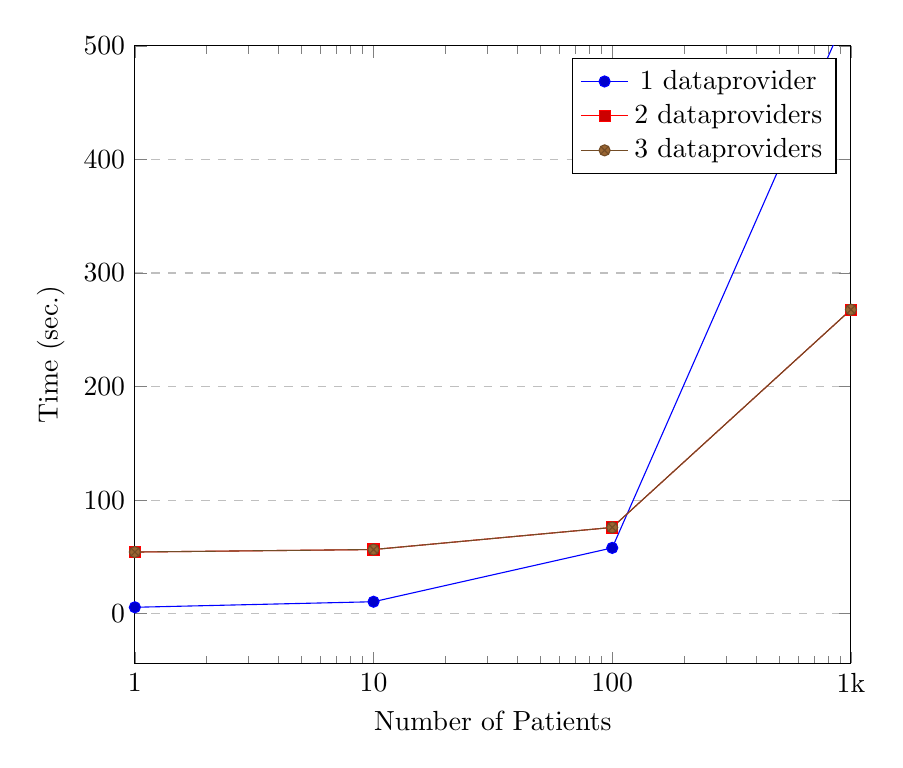
\begin{tikzpicture}
  \begin{axis}[scale only axis, enlarge x limits=-1, width=\textwidth*0.75, ymajorgrids=true, xmode=log, log ticks with fixed point, xlabel={Number of Patients}, ylabel={Time (sec.)}, xticklabels={1,10,100,1k}, ymax=500, grid style=dashed]
  \addplot
      coordinates {(1, 5.66)(10, 10.54)(100, 57.94)(1000, 536.09)};
  \addlegendentry{1 data\hyp provider}
  \addplot
      coordinates {(1, 54.29)(10, 56.5)(100, 75.95)(1000, 267.7)};
  \addlegendentry{2 data\hyp providers}
  \addplot
      coordinates {(1, 54.29)(10, 56.5)(100, 75.95)(1000, 267.7)};
  \addlegendentry{3 data\hyp providers}
  \end{axis}
  \end{tikzpicture}
  \caption{1-Dimensional numerical histograms timings for different number of data\hyp providers}
\end{minipage}%
\begin{minipage}{.5\linewidth}
  \centering
  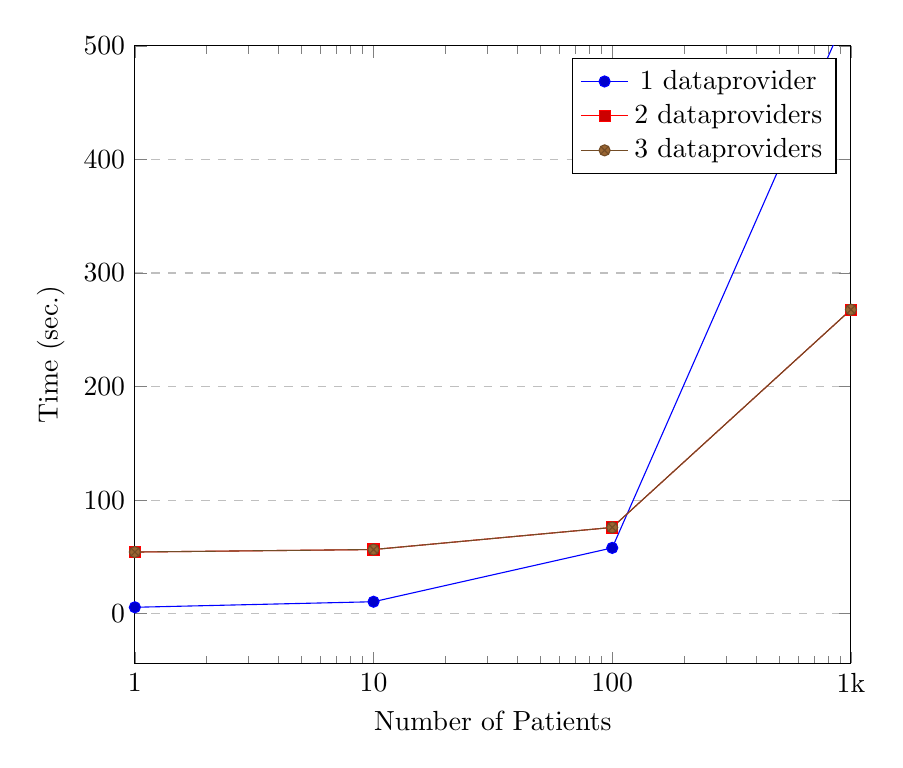
\begin{tikzpicture}
  \begin{axis}[scale only axis,enlarge x limits=-1,width=\textwidth*0.75,ymajorgrids=true,xmode=log,log ticks with fixed point,xlabel={Number of Patients},ylabel={Time (sec.)},xticklabels={1,10,100,1k},ymax=500,grid style=dashed]
  \addplot
      coordinates {(1, 5.66)(10, 10.54)(100, 57.94)(1000, 536.09)};
  \addlegendentry{1 data\hyp provider}
  \addplot
      coordinates {(1, 54.29)(10, 56.5)(100, 75.95)(1000, 267.7)};
  \addlegendentry{2 data\hyp providers}
  \addplot
      coordinates {(1, 54.29)(10, 56.5)(100, 75.95)(1000, 267.7)};
  \addlegendentry{3 data\hyp providers}
  \end{axis}
  \end{tikzpicture}
  \caption{2-Dimensional categorical histograms timings for different number of data\hyp providers}
\end{minipage}
}
\end{figure}



%%%%%%%%%%%%%%%%%%%%%%%%%%%%%%%%%%%%%%%%%%%%%%%%%%%%%%%%%%%%%%%%%%%%%%%%%%%%%%%%%%%
%%%%%%%%%%%%%%%%%%%%%%%%%%%%%%%%%%%%%%%%%%%%%%%%%%%%%%%%%%%%%%%%%%%%%%%%%%%%%%%%%%%
%%%%%%%%%%%%%%%%%%%%%%%%%%%%%%%%%%%%%%%%%%%%%%%%%%%%%%%%%%%%%%%%%%%%%%%%%%%%%%%%%%%

\subsection{Decision Trees}\label{ss:results-dtrees}

